\begin{tehtavasivu}

% FIXME: Tee vielä toinen tehtävä perusarvosta ``Kirjan myyntihinta'' -tehtävän lisäksi
% FIXME: laaja tehtävä ansio- ja pääomatulojen verotuksesta
\subsubsection*{Opi perusteet}

\begin{tehtava}
Täydennä taulukko.\\
\begin{tabular}{|c|c|c|c|}
\hline 
desimaaliluku & murtoluku & \% & \permil \\ 
\hline 
$0,1$ & &$10$ & \\ 
\hline 
 & $-\frac{4}{5}$ & & \\ 
\hline 
 & & $99,9$ & \\ 
\hline 
 & & & $0,42$ \\ 
\hline 
 & & $125$ & \\ 
 \hline
$-7,5$  & & & \\
  \hline
\end{tabular}
	\begin{vastaus}
\begin{tabular}{|c|c|c|c|}
\hline 
desimaaliluku & murtoluku & \% & \permil \\ 
\hline 
$0,1$ & $\frac{1}{10}$&$10$ &$100$ \\ 
\hline 
$-0,8$ & $-\frac{4}{5}$ & $-80$ & $-800$\\ 
\hline 
$0,999$ & $\frac{999}{1\,000}$& $99,9$ & $999$\\ 
\hline 
$0,00042$ &$\frac{21}{50\,000}$ & $0,042$& $0,42$ \\ 
\hline 
$1,25$ &$\frac{5}{4}$ & $125$ & $1\,250$\\ 
 \hline
$-7,5$ & $-\frac{15}{2}$& $-750$&$-7\,500$ \\
  \hline
\end{tabular}
	\end{vastaus}
\end{tehtava}

\begin{tehtava}
Täydennä taulukko. \\
\begin{tabular}{|c|c|c|} %epäkoherenssi sarakeotsikossa
\hline 
perusarvo & $\pm p$\,\% & lauseke \\ 
\hline 
$a$ & $+10$\,\% & $1,10a$ \\ 
\hline 
$b$ & $-24$\,\% & \\ 
\hline 
$5\,000$\,€ & $-1$\,\% & \\ 
\hline 
 & & $0,42x$ \\ 
\hline 
 $3$\,m& & $26\cdot 3$\,m \\ 
\hline
  & &$0,003\cdot(-7,5)$ \\
\hline
\end{tabular}
	\begin{vastaus}
\begin{tabular}{|c|c|c|}
\hline 
perusarvo & $\pm p$\,\% & lauseke \\ 
\hline 
$a$ & $+10$\,\% & $1,10a$ \\ 
\hline 
$b$ & $-24$\,\% &$0,76b$ \\ 
\hline 
$5\,000$\,€ & $-1\,\%$ &$0,99\cdot5\,000\,$€ \\ 
\hline 
$x$ &$-58\,\%$ & $0,42x$ \\ 
\hline 
 $3$\,m&$+2\,500\,\%$ &$26\cdot3$\,m \\ 
 \hline
 $-7,5$ & $-99,7\,\%$ & $0,003\cdot(-7,5)$ \\
  \hline %ehkä lisää rivejä :)
\end{tabular}

Huom.: $0,42x$ voidaan tulkita myös niin, että perusarvo on $0,42$ ja $x$ on prosenttikerroin (muotoa $1\pm \frac{p}{100})$. Sama tulkinnanvaraisuus koskee viimeisen rivin lauseketta $0,003\cdot (-7,5)$
	\end{vastaus}
\end{tehtava}

\begin{tehtava}
    Laske
    \alakohdat{
	  § $4,5\,\%$ luvusta $1\,500$
	  § $4,5\,\%$ luvusta $b$
	  § $15,3\,\%$ luvusta $b$
	  § $152\,\%$ luvusta $b$
	  § $3\,550\,\%$ luvusta $b$.
    }
    \begin{vastaus}
	  \alakohdat{
		§ $67,5$
		§ $0,045b$
		§ $0,153b$
		§ $1,52b$
		§ $35,5b$
	  }
    \end{vastaus}
\end{tehtava}

\begin{tehtava}
    Kuinka monta prosenttia
    \alakohdat{
	  § $15$ on luvusta $75$
	  § $120$ on luvusta $80$
	  § $400$ on luvusta $3,5$
	  § luku $50$ on lukua $170$ pienempi
	  § luku $170$ on lukua $50$ suurempi
	  § $400$ on lukua $3,5$ suurempi?
    }
    \begin{vastaus}
	  \alakohdat{
		§ $20$\,\%
		§ $150$\,\%
		§ $11\,428,6$\,\%
		§ $70,6$\,\%
		§ $240$\,\%
		§ $11\,328,6$\,\%
	  }
    \end{vastaus}
\end{tehtava}

\begin{tehtava}
    Oppikirjamaraton-tiimi kävi lounastamassa. Osoita oheisen kuitin tiedoilla vääräksi yleinen virhekäsitys, että $13\,\%$ suuruisen arvonlisäveron osuus olisi $13\,\%$ lopullisesta myyntihinnasta.
    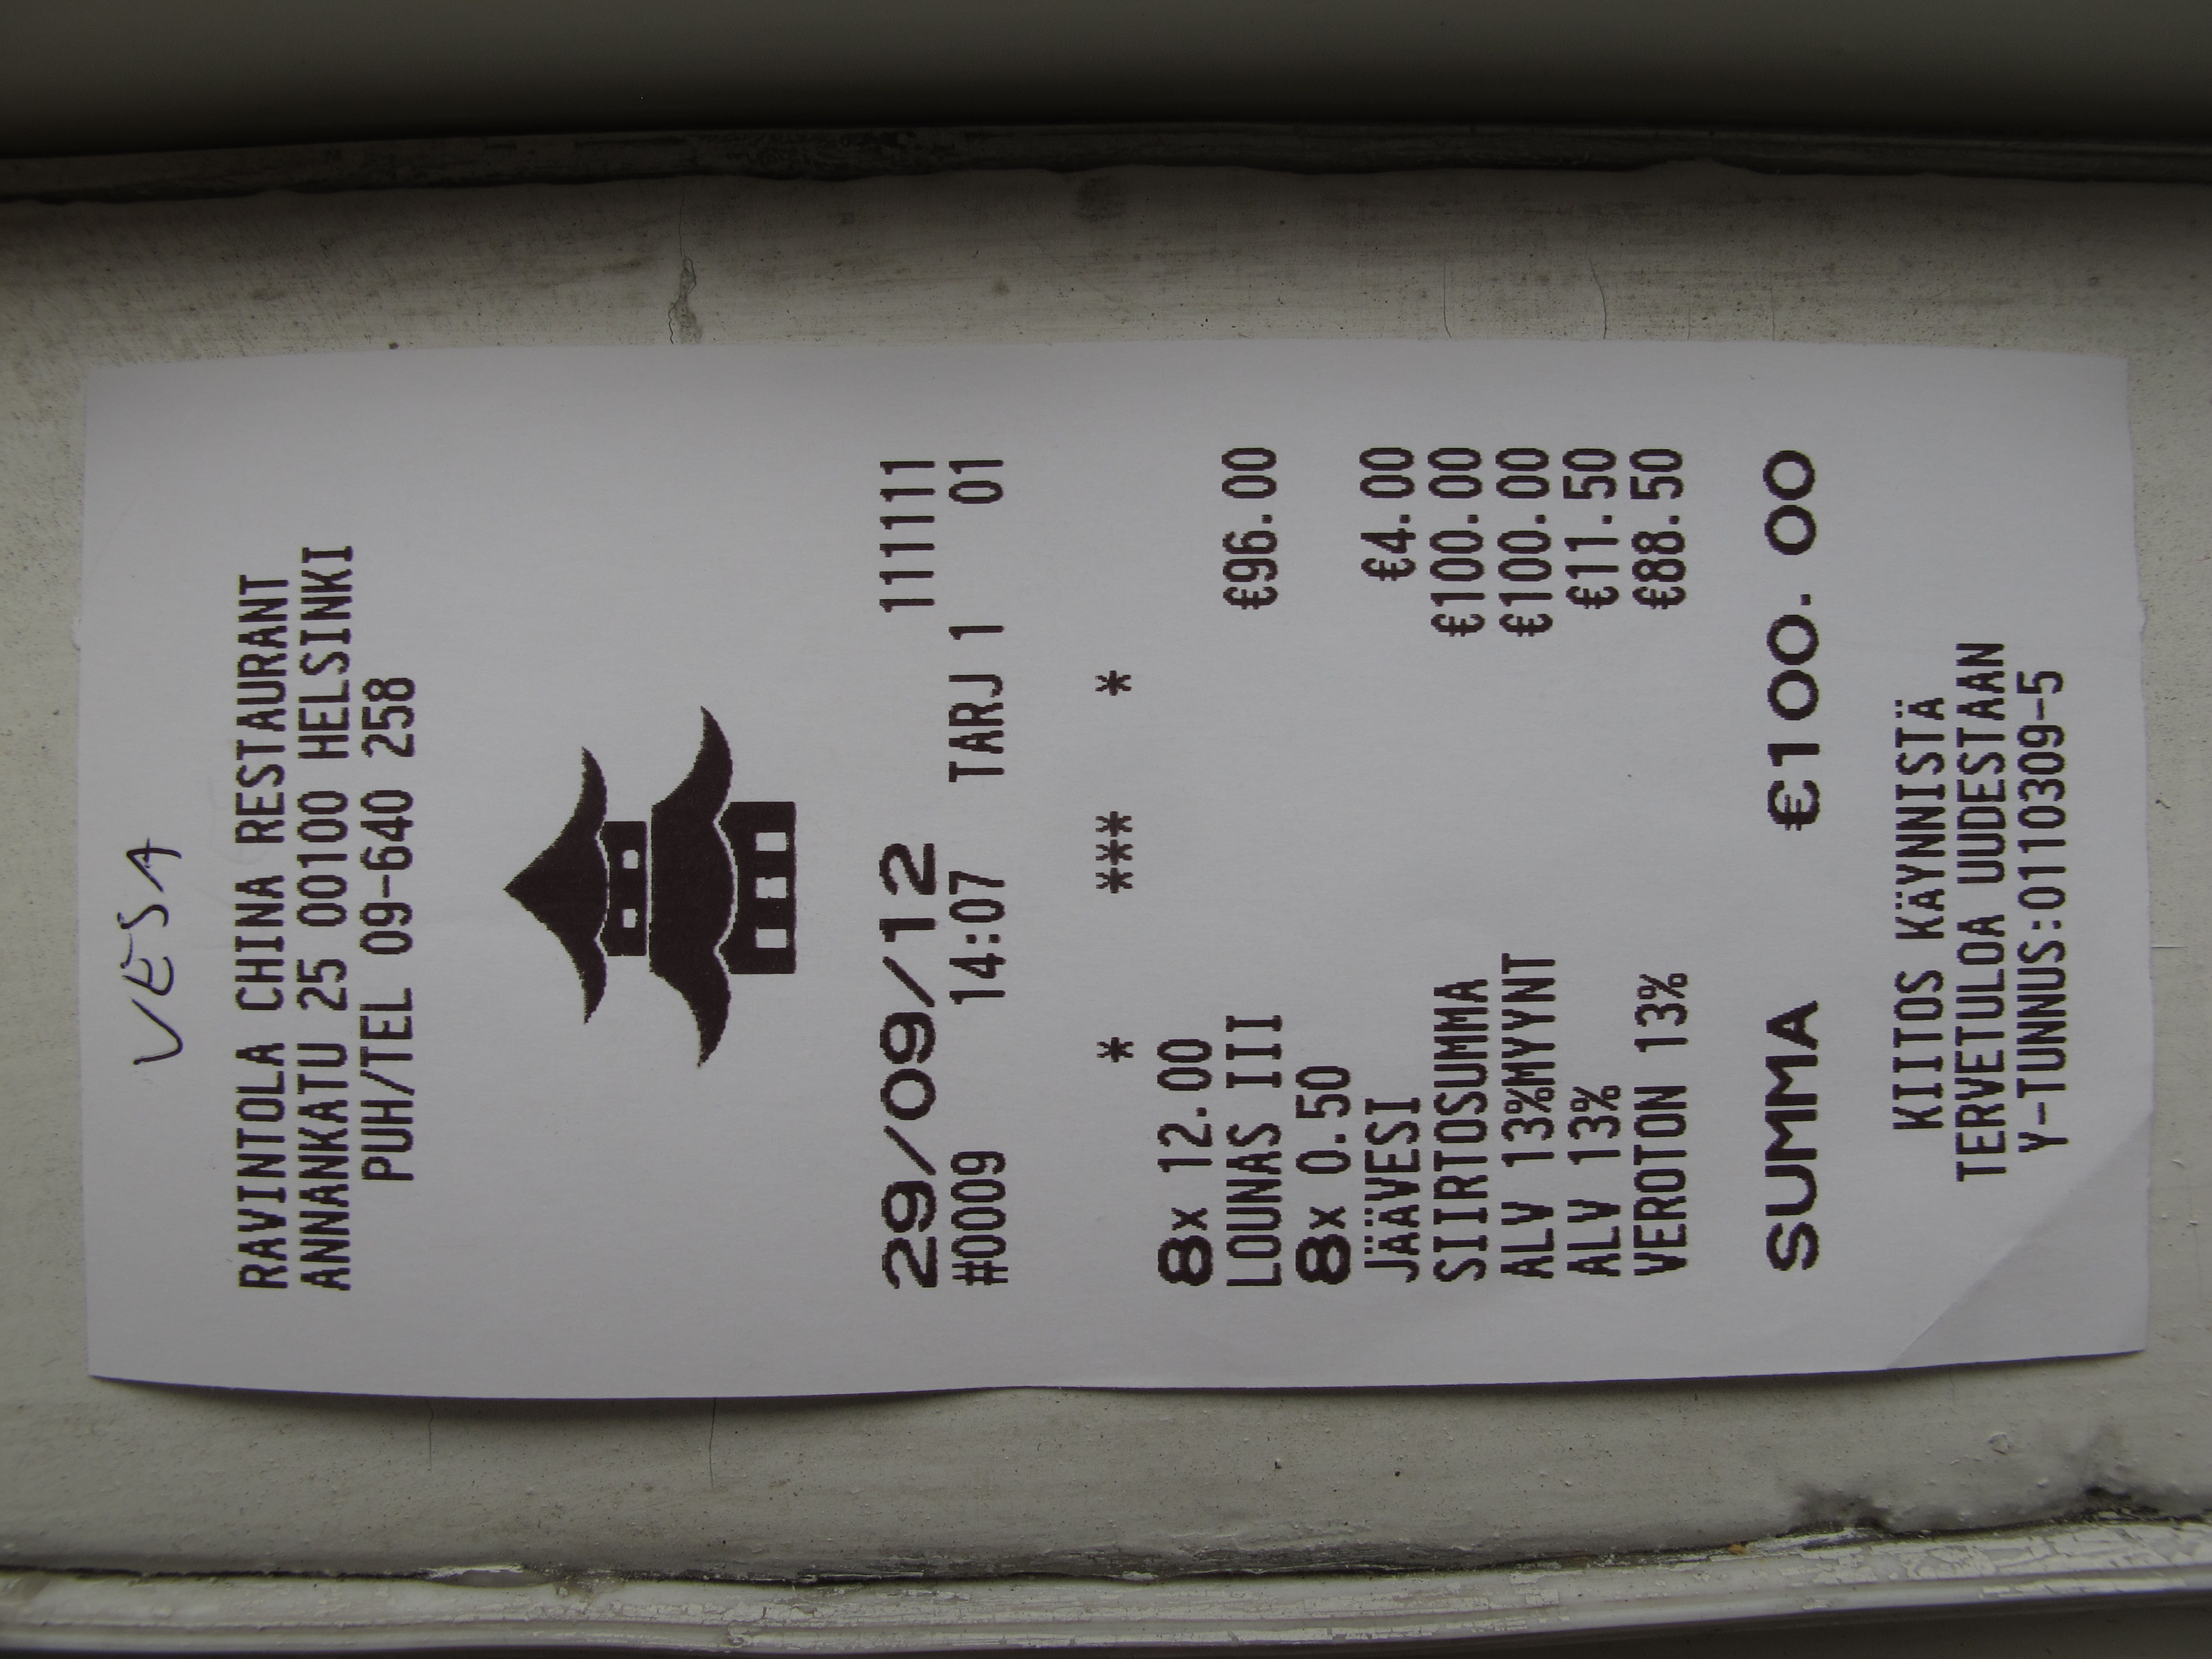
\includegraphics[width=80mm, angle=270]{pictures/alv-kuitti}
    \begin{vastaus}
         $13\,\%$ sadasta eurosta on $13$ euroa -- ei $11,50$ euroa, niin kuin kuitissa todetaan. Arvonlisävero lasketaan suhteessa verottomaan hintaan, ei lopulliseen myyntihintaan.
    \end{vastaus}
\end{tehtava}

\begin{tehtava}
    Laukun normaalihinta on $225$ euroa, ja se on $25$ prosentin alennuksessa. Mikä on alennettu hinta?
    \begin{vastaus}
        $168,75$ euroa
    \end{vastaus}
\end{tehtava}

\begin{tehtava}
    Jaakon kuukausipalkka on $1\,623,52$ euroa. Hän saa $1,3\,\%$ palkankorotuksen. Mikä on Jaakon kuukausipalkka korotuksen jälkeen?
    \begin{vastaus}
        $1\,644,63$ euroa
    \end{vastaus}
\end{tehtava}

\begin{tehtava}
Vuosien 2008 ja 2012 kunnallisvaaleissa ehdokkaita asettaneiden eduskunnan ulkopuolisten puolueiden saamat äänet koko maassa on esitetty seuraavassa taulukossa. Mukana ovat vain ne puolueet, jotka olivat mukana molemmissa vaaleissa. \\
\begin{tabular}{|c|c|c|}
\hline 
Puolue / Äänet & 2008 & 2012 \\ 
\hline
Itsenäisyyspuolue & $1\,482$ & $1\,303$ \\
\hline
\vtop{\hbox{\strut Kommunistinen}\hbox{\strut Työväenpuolue}}  & $1\,065$ & $704$ \\
\hline
Köyhien Asialla & $1\,059$ & $572$ \\ 
\hline
\begin{tabular}[x]{@{}c@{}}Suomen Kommunistinen\\Puolue\end{tabular} & $13\,986$ & $11\,174$ \\ 
\hline 
Suomen Työväenpuolue & $703$ & $538$ \\ 
\hline 
\end{tabular}
\alakohdat{
§ Minkä puolueen kannatus laski eniten äänissä laskettuna ja kuinka paljon?
§ Minkä puolueen äänisaalis laski eniten prosentuaalisesti ja kuinka paljon?
}
	\begin{vastaus}
	\alakohdat{
	§ Suomen Kommunistisen Puolueen, $2\,812$ ääntä
	§ Köyhien asialla -puolueen, $46$\,\%
	}
	\end{vastaus}
\end{tehtava}

\begin{tehtava} %lähde: Vaalit.fi
    Piraattipuolueen kannatus oli vuoden 2011 eduskuntavaaleissa $0,5\,\%$ ja vuoden 2014 europarlamenttivaaleissa $0,7\,\%$.
    \alakohdat{
    § Kuinka monta prosenttiyksikköä kannatus kasvoi? (Tiedotusvälineissä kannatusmuutokset ilmoitetaan yleensä prosenttiyksiköissä.)
    § Kuinka monta prosenttia kannatus kasvoi?
    }
    \begin{vastaus}
        \alakohdat{
        § Kannatus kasvoi $0,2$ prosenttiyksikköä.
        § Kannatus kasvoi $40$ prosenttia.
        }
    \end{vastaus}
\end{tehtava}

\begin{tehtava}
    Samulin pituus on $165$\,cm ja Joonaksen $173$\,cm.
    \alakohdat{
        § Kuinka monta prosenttia Samulin pituus on Joonaksen pituudesta?
        § Kuinka monta prosenttia Joonaksen pituus on Samulin pituudesta?
        § Kuinka monta prosenttia Samuli on lyhyempi kuin Joonas?
        § Kuinka monta prosenttia Joonas on pidempi kuin Samuli?
    }
    \begin{vastaus}
        \alakohdat{
            § $95,4\,\%$
            § $104,8\,\%$
            § $4,62\,\%$
            § $4,85\,\%$
        }
    \end{vastaus}
\end{tehtava}

\begin{tehtava}
    Jalkapalloilija Georgios Samaras teki ensimmäisellä kaudellaan Skotlannin valioliigassa (2007--2008) $5$ maalia Celtic F.\,C.:n paidassa. Seuraavalla kaudella Samaras teki Celticille liigassa $15$ maalia. Kuinka monta prosenttia Samaraksen maalimäärä nousi?
    \begin{vastaus}
        $200\,\%$
    \end{vastaus}
\end{tehtava}

\begin{tehtava}
    Erään pankin myöntämä opintolaina kasvaa korkoa $2\,\%$ vuodessa. Kuinka monta prosenttia laina on kasvanut korkoa alkuperäiseen verrattuna kymmenen vuoden kuluttua?
    \begin{vastaus}
        $22\,\%$
    \end{vastaus}
\end{tehtava}

\begin{tehtava}
    Kirjan myyntihinta, joka sisältää arvonlisäveron, on $9\,\%$ suurempi kuin kirjan veroton hinta. Laske kirjan veroton hinta, kun myyntihinta on $27$ euroa.
    \begin{vastaus}
        Kirjan veroton hinta on $24,77$ euroa.
    \end{vastaus}
\end{tehtava}

\begin{tehtava}
    Sokerijuurikkaassa on $18\,\%$ sokeria. Kuinka paljon sokerijuurikkaita (tonneissa) tarvitaan valmistettaessa $8$ tonnia sokeriliuosta, jonka sokeripitoisuus on $4,5\,\%$?
    \begin{vastaus}
        $2$ tonnia
    \end{vastaus}
\end{tehtava}

\begin{tehtava}
    Iidan ja Matin duo saa julkisuutta, ja he alkavat myydä CD-levyään keikkojen yhteydessä $10$ euron kappalehinnalla. Jonkin ajan päästä he päättävät nostaa CD-levyn hintaa $20$ prosenttia. Matti alkaa kuitenkin katua päätöstä, ja ehdottaa tämän korotetun hinnan alentamista $20$ prosentilla, jotta useampi levy saataisiin myytyä.
    \alakohdat{
    § Mikä olisi tämän toimenpiteen jälkeen CD:n uusi hinta?
    § Montako prosenttia olisi alennuksen oltava, jotta oikeasti päästäisiin takaisin alkuperäiseen $10$ euron hintaan?
    }
    \begin{vastaus}
    \alakohdat{
    § Uusi hinta on $9,60$ euroa.
    § Vaadittava alennus on $17\,\%$.
    }
    \end{vastaus}
\end{tehtava}

\subsubsection*{Hallitse kokonaisuus}

\begin{tehtava}
Paranoidi perheenäiti ei ole opiskellut suuruusluokkia, ja hänellä menee millit ja mikrot sekaisin. Kuinka monta prosenttia liian suuren annoksen hän saa, kun hän syö ravintolisänä eräänä päivänä D-vitamiinia $50$ mikrogramman sijasta $50$ milligrammaa? (Vihje: älä yritä tätä kotona.)
	\begin{vastaus}
 Hän saa $999$ prosenttia liian suuren annoksen.
	\end{vastaus}
\end{tehtava}

%http://www.paihdelinkki.fi/alkoholineuvonnan-opas/promille

\begin{tehtava}
    Hedelmissä on vettä aluksi $60\,\%$ niiden painosta. Kuinka monta prosenttia vedestä on haihdutettava, jotta hedelmissä tämän jälkeen olisi vain $20\,\%$ vettä?
    \begin{vastaus}
        $\approx83,3\,\%$ %pitää kertoa jossain, miten tuo ilmaisu luetaan...
    \end{vastaus}
\end{tehtava}

%kovalevytilan hävikkitehtävä

\begin{tehtava}
    (YO 2000K/4) Tuoreissa omenissa on vettä $80\,\%$ ja sokeria $4\,\%$. Kuinka monta prosenttia sokeria on samoissa omenissa, kun ne on kuivattu siten, että kosteusprosentti on $20$?
    \begin{vastaus}
        $16\,\%$
    \end{vastaus}
\end{tehtava}

\begin{tehtava}
Eräällä kuvitteellisella saarella on vain kaksi valtiota: X ja Y. Valtioissa oli saman verran asukkaita, kunnes niiden välille syttyi sota. Tuhoisan ja hyvin yksipuolisen sodan seurauksena valtion Y asukasmäärä putosi sadasosaan entisestä, ja valtion X asukasmäärä putosi viisi prosenttia.
\alakohdat{
§ Esitä kokonaislukujen suhteena valtioiden sodan jälkeiset asukasmäärät.
§ Kuinka monta prosenttia valtion Y sodanjälkeinen asukasmäärä on koko saaren sodanjälkeisestä asukasmäärästä? Anna vastaus prosentin sadasosien tarkkuudella.
§ Kuinka monta prosenttia saaren asukasmäärä väheni sodan seurauksena?
}
	\begin{vastaus}
	\alakohdat{
	§ $95:1$
	§ $1,04\,\%$
	§ Olkoon $a$ valtion X tai Y alkuperäinen populaatio (sama molemmissa), jolloin saaren alkuperäinen populaatio on $2a$. Uusi asukasmäärä on $0,01\cdot a+0,95\cdot a$. Laskemalla vanhan ja uuden saaripopulaation erotus verrattuna alkuperäiseen saadaan: $\frac{2a-(0,01\cdot a+0,95\cdot a)}{2a}=\frac{2a-0,01a-0,95a}{2a}=\frac{1,04a}{2a}=\frac{1,04}{2}=0,52=52\,\%$. (Voi toki myös laskea vain uuden ja vanhan suhteen ja päätellä siitä tuloksen.)
	}
	\end{vastaus}
\end{tehtava}

\begin{tehtava}
    Askartelukaupassa on alennusviikot ja kaikki tavarat myydään $60\,\%$:n alennuksella. Viimeisenä päivänä kaikista hinnoista annetaan vielä lisäalennus, joka lasketaan aiemmin alennetusta hinnasta. Minkä suuruinen lisäalennus tulee antaa, jos lopullisen kokonaisalennuksen halutaan olevan $80\,\%$?
    \begin{vastaus}
        $50\,\%$
    \end{vastaus}
\end{tehtava}

\begin{tehtava}
	Avoin kierros laserhippaa (laser tag) maksaa yhdeltä pelaajalta $9$ euroa. Pelialueen voi kuitenkin varata seurueelle hintaan $260$ euroa. Mette on menossa pelaamaan viiden kaverinsa kanssa. 
	\alakohdat{
		§ Kuinka monta prosenttia kalliimpaa on varata joukolle yksityispeli kuin liput avoimeen peliin?
		§ Kuinka suuri seurueen on vähintään oltava, jotta yksityispeli tulisi halvemmaksi?
	}
	\begin{vastaus}
		\alakohdat{
			§ $381\,\%$
			§ $29$
		}
	\end{vastaus}
\end{tehtava}

\begin{tehtava}
    Vuonna 2012 yleinen arvonlisäveroprosentti Suomessa oli $23\,\%$ tuotteen verottomasta hinnasta. Tuotteen hinta koostuu sen verottomasta hinnasta ja tuotteesta maksettavasta arvonlisäverosta. Kuinka monta prosenttia arvonlisävero on tuotteen myyntihinnasta?
    \begin{vastaus}
        $18,7\,\%$
    \end{vastaus}
\end{tehtava}

\begin{tehtava}
    Kun matkalipun hintaa korotettiin $10,0\,\%$, matkustajien määrä väheni $10,0\,\%$. Kuinka monella prosentilla tällöin kasvoivat tai vähenivät liikennöitsijän lipputulot?
    \begin{vastaus}
        Lipputulot vähenivät $1$ prosentilla.
    \end{vastaus}
\end{tehtava}

\begin{tehtava}
Jos geenitekniikan laboratoriossa käsitellään tai tutkitaan RNA:ta, täytyy kyseistä DNA:n sukulaismolekyyliä tuhoavat entsyymit deaktivoida. Dietyylipyrokarbonaatti (DEPC) on voimakas proteiineja denaturoiva ja sakkaava yhdiste, ja sopii tähän tarkoitukseen hyvin. Tavallinen ohje tarvittavan puhdistusliuoksen valmistamiseen on, että valmista $100$ prosentin DEPC-liuosta laimennetaan $94$-prosenttisella etanolilla $10$-prosenttiseksi. Etanoli on laimennettu puhtaalla vedellä. Kuinka paljon vettä on $500$ millilitrassa valmista käyttöliuosta? Jokainen ilmoitettu prosentuaalinen arvo on \termi{tilavuusprosentti}{tilavuusprosentti} eli kunkin komponentin tilavuuden suhde koko liuoksen tilavuuteen.
	\begin{vastaus}
	Valmiista liuoksesta $10\,$\% on DEPC:tä ja $90\,$\% laimennettua etanolia, josta $94\,$\% on etanolia ja $6$\,\% vettä. Vettä on siis $0,06\cdot0,90\cdot500$\,ml$=27$\,ml.
	\end{vastaus}
\end{tehtava}

\begin{tehtava}
Suomalaisista masennuspotilaista arviolta jopa $30$\,\%:lla on samanaikainen alkoholiongelma, ja alkoholista riippuvaisista arviolta jopa $60$\,\%:lla on kliinisesti merkittävä depressio.
	\alakohdat{
	§ Kuinka suuri osa masentuneista suomalaisista ei ole alkoholiongelmaisia (alkoholiriippuvaisia)?
	§ Kuinka suuri osa alkoholiongelmaisista (alkoholiriippuvaisista) suomalaisista ei ole masentuneita?
%	§ Kumpia on suomalaisista enemmän: masentuneita vai alkoholiongelmaisia?
	}
	\begin{vastaus}
		\alakohdat{
	§ $70$\,\%
	§ $40$\,\%
%	§ 
	}
	\end{vastaus}
\end{tehtava}

\subsubsection*{Lisää tehtäviä}

%Lisännyt Aleksi Sipola 10.11.2013
\begin{tehtava}
    (YO 1991K/5a) Luvun $\sqrt{r^2-a^2}$ likiarvona voidaan käyttää lukua $r-{\frac{1}{2}a^2}/r$. Laske tämän nojalla $\sqrt{3}$ likiarvo sopivia kokonaislukuja $r$ ja $a$ käyttäen. Kuinka monta prosenttia tämä likiarvo poikkeaa tarkasta arvosta?
    \begin{vastaus}
        Likiarvo on $1,75$ ja $\sqrt{3}=1,732\ldots$ Likiarvo poikkeaa noin $1,04\,\%$.
    \end{vastaus}
\end{tehtava}

\begin{tehtava}
    (YO 1877/4) Kaupungissa tuli jokaisen talonomistajan suorittaa kaupungin kassaan $5\,\%$ saadusta hyyrymäärästä (vuokrasta, ruotsin sanasta \textit{hyra}). Sittemmin määrättiin, että mainittu prosentti oli oleva $10$. Monellako prosentilla talonomistajien täytyi korottaa hyyryjä saadakseen saman puhtaan säästön kuin ennen?
    \begin{vastaus}
        $5,6\,\%$
    \end{vastaus}
\end{tehtava}
	
\begin{tehtava}
Miksi ei kannata mennä ostoksille kauppaan, joka mainostaa liikkeessä olevan ''$-40$\,\%:n alennus''?
	\begin{vastaus}
	Pelkkä ''$40$ prosentin alennus'' tarkoittaa, että hinnat on kerrottu prosenttikertoimella $1-\frac{40}{100}=0,6$. Jos kyseessä on negatiivinen alennus, prosenttikerroin on $1-\frac{-40}{100}=1+\frac{40}{100}=1,4$, eli hintoja on kasvatettu!!!!11
	\end{vastaus}
\end{tehtava}	

\begin{tehtava} 
		$\star$ Luolassa asuu $99$ ihmistä. Aikuisia on $50\,\%$ vähemmän kuin lapsia. Montako aikuista luolassa asuu?
	\begin{vastaus}
	Luolassa asuu $33$ aikuista.
	\end{vastaus}
\end{tehtava}

\end{tehtavasivu}